% couette-flow-2D.tex

\newpage
\section{Couette Flow: 2D}
\label{couette-flow-2D}
%
This case computes the flow between two parallel plates,
one is a moving wall with a translational velocity while the other stationary wall.
The flow is driven by the virtue of viscous darg force acting on the fluid and the applied
pressure gradient parallet to the plates.This test case is used to verify the translational
velocity of the newly defined moving wall boundary condition.

\begin{figure}[htbp]
\begin{center}
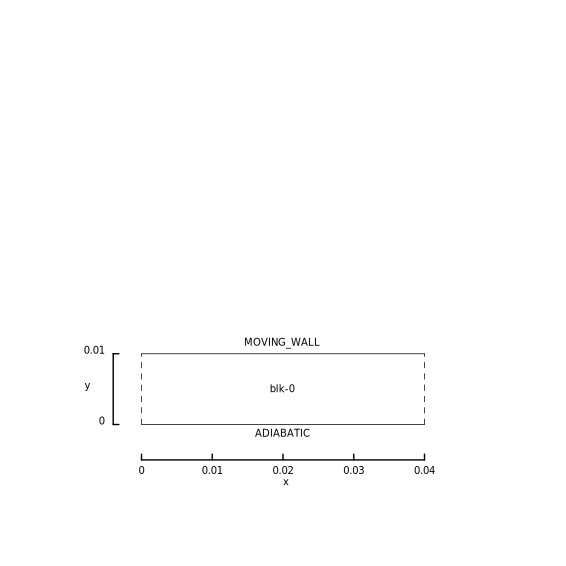
\includegraphics[width=0.5\textwidth,viewport=139 274 503 629,clip=true]{../2D/couette-flow/couette.pdf}
\end{center}
\caption{Flow domain for viscous flow between two parallel plates.}
   \label{couette-layout-fig}
\end{figure}

\medskip
First, a two dimensional couette flow is studied, and the boundary condition is shown in Figure~\ref{couette-layout-fig}.
The NORTH and SOUTH face are set as the Moving Wall and Adiabatic boundary condition, respectively, while the function of 
\texttt{connect\_blocks\_2D} is used to connect the WEST and EAST faces, which can be regarded as
Periodic boundary condition.

\begin{figure}[htbp]
\begin{center}
\includegraphics[width=0.6\textwidth]{../2D/couette-flow/c_2D_mesh.png}
\end{center}
\caption{Mesh profile for two dimensional couette flow.}
   \label{couette-mesh-fig}
\end{figure}

\begin{figure}[htbp]
\begin{center}
\includegraphics[width=0.6\textwidth]{../2D/couette-flow/c_2D_velocity_counter.png}
\end{center}
\caption{Velocity contour for two dimensional couette flow.}
   \label{couette-velocity-fig}
\end{figure}

\medskip
And, a mesh of $20 \times 10$ is plotted in Figure~\ref{couette-mesh-fig}. The velocity of the NORTH face is set as $100 m/s$
at the $y$ direction, since the data extracted is the central cell closed to the face, it might be a little bit less than the velocity 
of moving wall. The velocity coutour can be shown in Figure~\ref{couette-velocity-fig}, the maximum velocity at $y$ direction 
is approximately 95$m/s$, slightly less than the translational velocity of moving wall.

\begin{figure}[htbp]
\begin{center}
\includegraphics[width=0.8\textwidth,viewport=38 49 422 302,clip=true]{../2D/couette-flow/velocity.pdf}
\end{center}
\caption{Velocity profile along the height.}
   \label{couette-velocityp-fig}
\end{figure}

\medskip
Since the initial velocity profile along the height is set as linear, the solution would achieve steady state condition quickly.
The final velocity profile is the same with the initial value, which is shown in Figure~\ref{couette-velocityp-fig}.

\newpage
\subsection{Input script (.py)}
\topbar
\lstinputlisting[language={}]{../2D/couette-flow/couette.py}
\bottombar


\subsection{Shell scripts}
\label{couette-flow-2D-sh-files}
\topbar
\lstinputlisting[language={}]{../2D/couette-flow/couette.sh}
\bottombar

\subsection{Notes}
\begin{itemize}
\item None
\end{itemize}


